\chapter{Resultados}

\drop{E}l objetivo de este capítulo es presentar de manera detallada los resultados obtenidos tras aplicar la metodología descrita en el capítulo anterior. El capítulo se encuentra estructurado por iteraciones y los resultados obtenidos en cada una de ellas.

\section{Resultado}

Tras finalizar el desarrollo de este proyecto se ha obtenido:

Un sistema de integración continua, implantado con éxito en la metodología de gestión del ciclo de desarrollo de \ac{Madrija} que permite gestionar el ciclo de pruebas de cualquier proyecto desde el principio hasta el final. Por lo tanto, se confirma haber alcanzado el objetivo principal definido en el capítulo 2 de este proyecto.

Dicho sistema de integración continua tiene la capacidad de realizar diferentes tareas:
\begin{itemize}
    \item Configura las variables de entorno necesarias para que se realice de manera correcta la compilación de los proyectos.
	\item Descargar el código fuente desde el repositorio donde trabaja el equipo de desarrollo.
    \item Utiliza las credenciales necesarias para poder descargarse el código fuente del respositorio.
	\item Una vez descargado el código fuente del proyecto, es capaz de elegir el \textit{branch} en el cual desea realizar las pruebas, es decir, en el proyecto ``X'' es capaz de elegir la rama ``Y'' correspondiente con el cliente ``Z'' y realizarle las pruebas que sean necesarias sólo a ese cliente.
	\item Es capaz de detectar cambios en el repositorio para comenzar la ejecución de los \textit{builds}.
    \item Establece una conexión \textit{maestro-esclavo} mediante el uso de \textit{Java Web Start} para permitir la comunicación entre el servidor de integración continua (maestro) y el equipo donde se van a realizar las ejecuciones (cliente).
    
    \clearpage
    
	\item El sistema de integración continua tiene la capacidad de realizar las compilaciones necesarias para cada proyecto, permitiendo así la integración de los diferentes artefactos e infraestructuras. Es decir, tiene la capacidad de compilar los proyectos padres necesarios para que el proyecto sobre el que se desea trabajar se compile de manera correcta.
	\item Mediante el uso de SSH es capaz de comunicar el servidor con los diferentes equipos.
	\item Es capaz de utilizar \textit{Vagrant} para crear máquinas virtuales de los diferentes sistemas operativos de cada cliente, incluyendo a cada sistema operativo su cofiguración correspondiente, permitiendo crear un clon lo más exacto posible del entorno de producción y tener así la capacidad de realizar las pruebas necesarias en un entorno con la mayor similitud posible al entorno real donde se ejecutará el software desarrollado.
    \item Es capaz de orquestar diferentes tecnologías como \textit{HSQLDB} o \textit{Liquibase} para preparar las bases de datos de prueba necesarias para la realización de pruebas sobre ellas.
    \item El sistema de integración continua es capaz de empaquetar y mover hacia un contenedor de aplicaciones, en este caso \textit{Apache Tomcat}, los archivos necesarios para ``levantar'' por completo el código fuente.
	\item Lanza la ejecución de los diferentes tipos de tests, tests unitarios, tests de comandos, tests de compatibilidad con los diferentes tipos de bases de datos, mediante el uso de ``Renombrator'' y tests de interfaz de usuario.
	\item Una vez han finalizado las pruebas, es capaz de destruir los elementos que ha creado para ejecutarlas, es decir, es capaz de destruir la máquina virtual nombrada antes para que el equipo vuelva a su estado anterior.
	\item Cuando el equipo ha vuelto al estado anterior, notifica mediante correo electrónico a todos los desarrolladores de cada proyecto, el estado en el cual se encuentra el proyecto, es decir, si el proyecto ha superado todos los tests o ha fallado en alguno test.
\end{itemize}

Por lo tanto, se ha desarrollado con éxito un sistema de integración continua capaz de realizar el ciclo completo de pruebas a cualquier proyecto de \ac{Madrija}. El sistema de integración continua cumple con todos los requisitos que han sido demandados por parte de la empresa durante las distintas reuniones en las distintas iteraciones.

\clearpage

En consecuencia, tras la implantación del sistema de integración continua, \ac{Madrija} ha obtenido una arquitectura e infraestructura donde se han implantado el sistema de integración continua, desde la cual se orquestan a las diferentes máquinas donde se realizan las pruebas necesarias.

\begin{figure}[!h]
\centering
   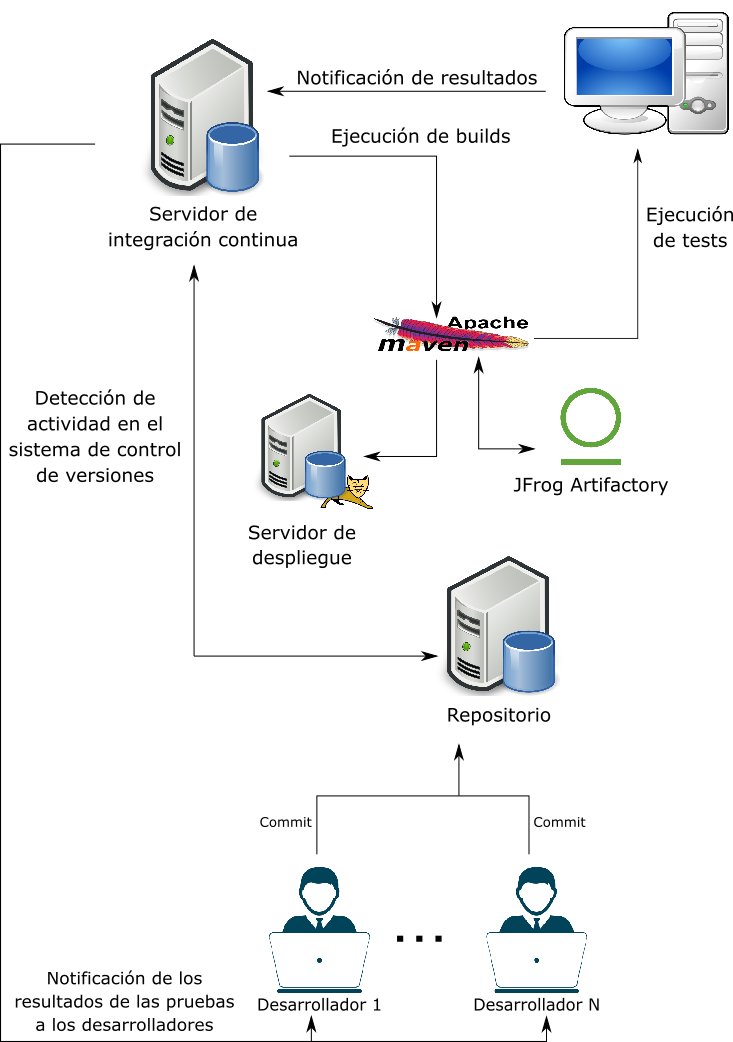
\includegraphics[width=12cm]{Prototipo_Sistema_IC.png}
\caption{Arquitectura e infraestructura del sistema de integración continua}
\end{figure}

La arquitectura e infraestructura permite al sistema de integración continua comunicarse con los diferentes equipos y servidores que utiliza \ac{Madrija}.

\clearpage

Por una parte, el desarrollador permanece aislado de lo que ocurre, simplemente desarrolla software y coloca todo lo necesario para realizar un \textit{build} en el repositorio (código fuente, \textit{scripts} de bases de datos, etcétera), dicho repositorio se encuentra en constante comunicación con el servidor de integración continua, en cuanto detecta un cambio en el repositorio (\textit{commit}, \textit{push}, etcétera), el servidor lanza las ejecuciones necesarias para realizar el ciclo completo de pruebas, orquesta dichas pruebas con Maven, descarga las librerías que necesite de \textit{JFrog Artifactory}, realiza las compilaciones necesarias para integrar los diferentes artefactos e infraestructuras y lanza la aplicación en el servidor de aplicaciones, finaliza las pruebas y envía los resultados al equipo de desarrollo.

Por otra parte, se ha obtenido una estrategia para lanzar las ejecuciones del servidor de integración continua, es decir, el servidor de integración continua detecta un cambio en el código fuente y lanza las ejecuciones para comprobar que esos cambios no violen ninguna restricción y mantenga el funcionamiento del código fuente de manera correcto.

El software ``Renombrator'' ha sido mejorado e integrado en el sistema de integración continua, este software permite migrar una base de datos de un tipo a otro.

\begin{figure}[!h]
\centering
   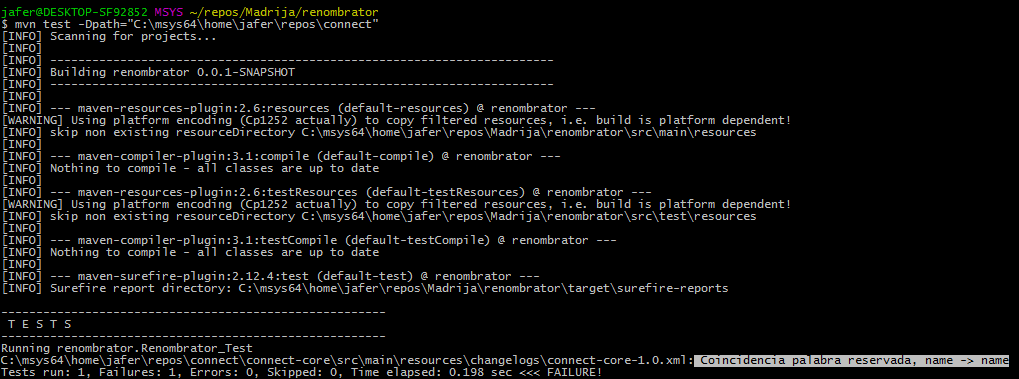
\includegraphics[width=15cm]{RenombratorResultado.PNG}
\caption{Ejecución y muestra de resultados de ``Renombrator''}
\end{figure}

Ees decir, comprueba que el código y los \textit{scripts} desarrollados para crear las bases de datos sean compatibles con bases de datos de PostgreSQL, Microsoft SQL Server, HSQLDB y Oracle. ``Renombrator'' es capaz de realizar pruebas como:

\begin{itemize}
	\item Comprobar que no se viole la restricción del número máximo de caracteres que puede tener un campo de una base de datos, es decir, si la longitud máxima es de 30 caracteres, que no se viole esa restricción.
	\item Comprueba que no se hace uso de palabras reservadas en cada tipo de base de datos.
	\item Comprueba que no se haga un uso incorrecto de mayúsculas y minúsculas.
\end{itemize}

\begin{figure}[!h]
\centering
   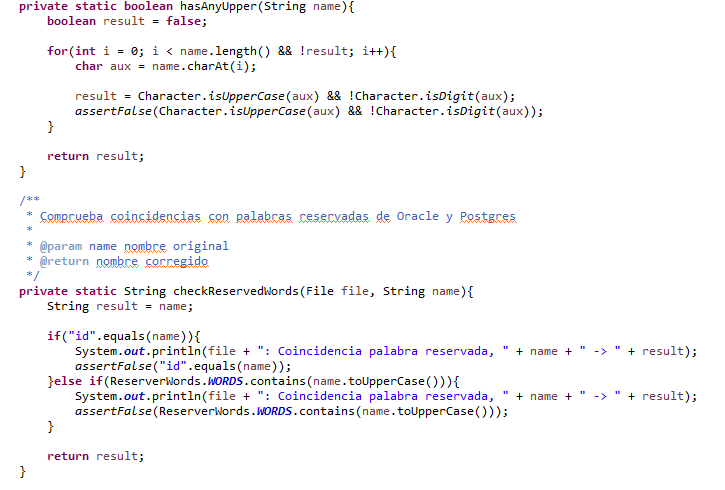
\includegraphics[width=15cm]{Renombrator.PNG}
\caption{Parte del código desarrollado para los tests de ``Renombrator''}
\end{figure}

\section{Iteraciones}

\subsection{Iteración 1}

En esta primera iteración se pretende obtener un prototipo del análisis, diseño, desarrollo e implantación del sistema de integración continua para varios proyectos reales de \ac{Madrija} obteniendo así una primera prueba de concepto, se va a seguir una metodología heurística, en concreto la metodología heurística IDEAL.

\subsubsection{Identificación del problema}

Se realiza una reunión con \ac{Madrija} y mediante el uso de diferentes técnicas de captura de requisitos, se capturan los requisitos que se persiguen en esta iteración y se aprueban estos requisitos mediante otra reunión con miembros de \ac{Madrija}, en esta iteración el objetivo principal consiste en desarrollar una prueba de concepto de un sistema de integración continua para proyectos reales de la empresa en un plazo de dos semanas. %dicho sistema de integración continua debe ser capaz de realizar el ciclo completo de los proyectos desde el principio a fin, es decir, desde descargar el código fuente de la aplicación desde el repositorio hasta ser capaz de desplegar y realizar pruebas sobre dicho código.

\subsubsection{Realización del plan}

Una vez obtenidos los requisitos del sistema que desea implantar \ac{Madrija}, se procede al análisis, diseño y desarrollo de un plan que permita abordar y solucionar los problemas identificados.

\clearpage

Entre los requisitos que \ac{Madrija} desea que tenga el sistema de integración continua destacan:
\begin{itemize}
\item Capacidad para descargar el código fuente desde el repositorio donde trabaja el equipo de desarrollo.
\item Capacidad para realizar las compilaciones necesarias, permitiendo así la integración entre los diferentes artefactos y la infraestructura.
\item Capacidad de comunicación con alguna herramienta para crear entornos virtuales.
\item Capacidad para ejecutar los tests necesarios para el código fuente descargado.
\item Capacidad de destruir los entornos virtuales y los elementos que ha creado para la ejecución de las pruebas.
\item Capacidad de comunicar a los miembros del equipo de desarrollo el resultado de las pruebas ejecutadas.
\end{itemize}

\subsubsection{Ejecución del plan}

En esta fase de la heurística IDEAL se llevan a cabo las tareas que se han marcado en la fase anterior para llegar al objetivo marcado.

%Una vez comprobada la viabilidad mediante una prueba de concepto, del sistema de integración continua con la metodología utilizada por la empresa para el ciclo de vida de sus productos se comprobará la compatibilidad entre el sistema de integración continua con las herramientas y tecnologías que utiliza \ac{Madrija}, en esta primera iteración se pondrá especial atención con el software de control de versiones (Git), los repositorios (GitLab), el lenguaje de programación utilizado para realizar los desarrollos (Java), la herramienta para la gestión y construcción de proyectos y sus dependencias (Apache Maven), las herramientas que permiten comunicar e interactuar con bases de datos (PostgreSQL, Liquibase y HSQLDB), la herramienta que permite la creación y configuración de entornos de desarrollo virtualizados (Vagrant) y la herramienta que permite ``levantar'' la aplicación en un contenedor de aplicaciones (Apache Tomcat).


\begin{figure}[!h]
\centering
   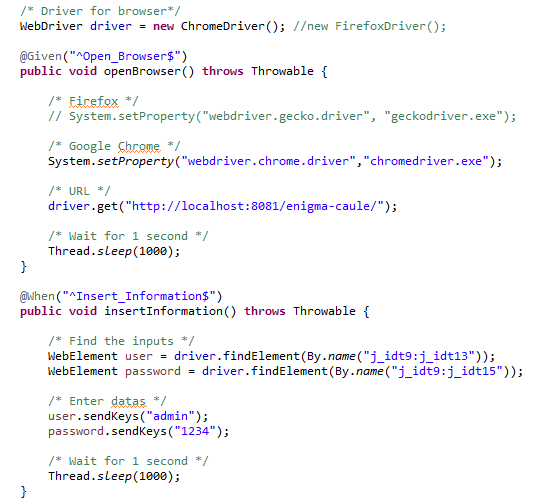
\includegraphics[width=9cm]{Test_Selenium_zz-caule.PNG}
\caption{Test desarrollado en Java con Selenium}
\end{figure}

%El sistema de integración continua habrá realizado todas sus acciones de manera correcta si consigue orquestar todas estas herramientas y tecnologías, sin errores, realizando los mismos pasos y obteniendo los mismos resultados que si todo el proceso se realizase de manera manual por algún desarrollador.

%Una vez obtenido todo lo anterior, se desarrollarán tests utilizando Selenium, se comprobará que los resultados obtenidos mediante el sistema de integración continua son iguales que los resultados obtenidos sin él, dado que los tests de Selenium serán ejecutados por el sistema de integración y él mismo mostrará los resultados obtenidos tras la finalización de la ejecución de los tests, permitiendo así al desarrollador recibir un correo electrónico informándole, entre otras cosas, de los resultados obtenidos en todo el proceso, desde la recuperación del código fuente del repositorio hasta la finalización de los tests o los cambios realizados por otros desarrolladores desde la última ejecución.
\clearpage

Finalizados todos los pasos desglosados del plan, se realizan tests y pruebas mediante el sistema de integración continua, obteniendo los mismos resultados que sin su implantación, es decir, los resultados obtenidos de las pruebas realizadas a los proyectos con o sin sistema de integración continua son iguales.

\subsubsection{Análisis de la solución obtenida}

Se realiza una reunión con miembros de \ac{Madrija} para presentarles la solución obtenida, se comentan los problemas que han surgido, \ac{Madrija} acepta la solución propuesta y se cierra esta primera iteración del proyecto. Como se ha dicho explicado antes, se toma el prototipo obtenido de esta iteración y se toma como entrada de la siguiente iteración.

\begin{figure}[!h]
\centering
   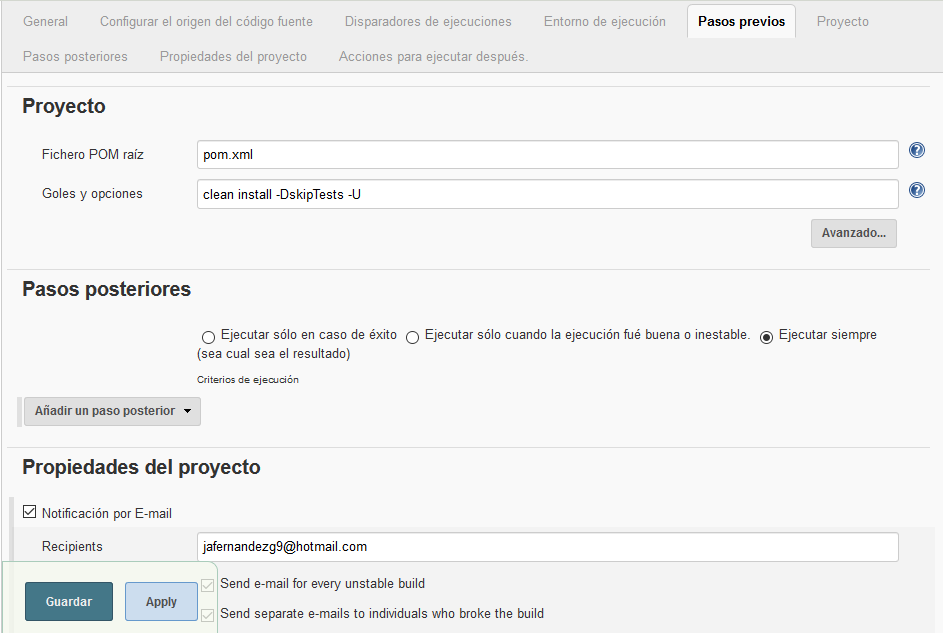
\includegraphics[width=14cm]{JenkinsMateriales.PNG}
\caption{Indicación de objetivos de un proyecto Maven en Jenkins}
\end{figure}

\subsubsection{Elección de la herramienta de integración continua}

Debido a la gran variedad de herramientas de integración continua en el mercado se realizó un estudio e investigación para elegir la opción que permita obtener más beneficio para \ac{Madrija}, en consecuencia, se elige Jenkins, debido a que es la herramienta que mejor se adapta a las tecnologías y herramientas utilizadas por \ac{Madrija}, contiene muchos plugins y, además, como plus añadido es una herramienta \textit{open source} y gratuita por lo que no supone ningún coste extra para la empresa. Jenkins superó la primera prueba de concepto.

\clearpage

Además, Jenkins cuenta con una serie de dibujos junto a los proyectos que contiene para informar de las estadísticas de los mismos.

\begin{itemize}
\item \textbf{Sol:} No hay ejecuciones recientes con fallos.
\item \textbf{Sol con nubes:} Una de las cinco últimas ejecuciones ha fallado.
\item \textbf{Nubes:} Dos de las cinco últimas ejecuciones han fallado.
\item \textbf{Lluvia:} Tres de las últimas cinco ejecuciones han fallado.
\item \textbf{Tormenta:} Cuatro de las cinco últimas ejecuciones han fallado.
\end{itemize}

\begin{figure}[!h]
\centering
   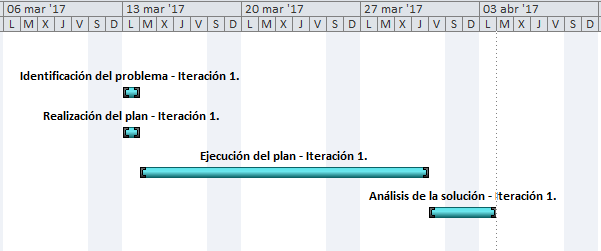
\includegraphics[width=9cm]{Diag-Gantt_It1.PNG}
\caption{Diagrama de Gantt de la iteración 1}
\end{figure}

\subsubsection{Problemas surgidos}

Debido a conflictos iniciales entre algunas librerías y herramientas el sistema de integración continua no podía contar el número de tests que ejecutaba, es decir, era capaz de determinar si se realizaban todos bien o si por el contrario algún test fallaba pero no era capaz de suministrar una cifra de tests bien ejecutados y de tests fallidos.

Por lo que debido al desconocimiento de estos problemas que surgieron durante el desarrollo, esta primera iteración duró tres semanas en lugar de las dos semanas que se estimaron inicialmente.

%\begin{figure}[!h]
%\centering
%   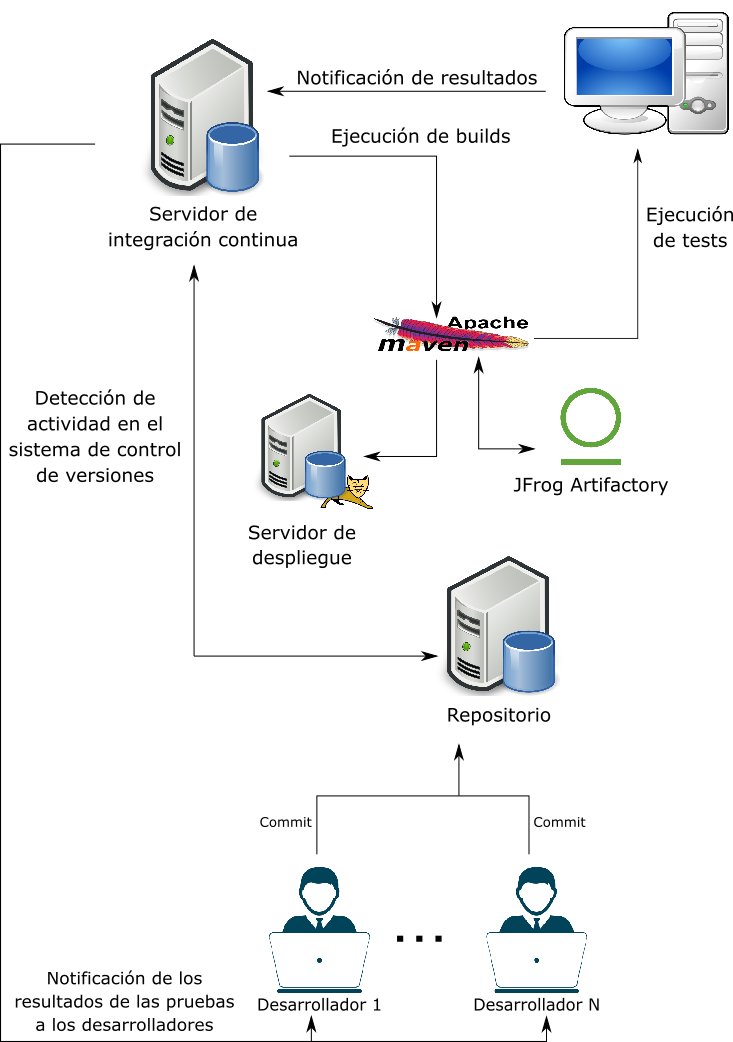
\includegraphics[width=12cm]{Prototipo_Sistema_IC.png}
%\caption{Sistema de integración continua}
%\end{figure}

\subsection{Iteración 2}

En esta segunda iteración mediante el análisis, diseño, desarrollo e investigación sobre sistemas de integración continua, se pretende definir un prototipo de una infraestructura y arquitectura para el sistema de integración continua que desea implantar \ac{Madrija}, para realizar esta segunda iteración, se va a utilizar una metodología heurística, en concreto la metodología heurística IDEAL.

\subsubsection{Identificación del problema}

Se lleva a cabo una reunión con \ac{Madrija}, donde se abordan la necesidad de determinar como debería ser la infraestructura y arquitectura que será necesaria para implantar un sistema de integración continua dentro de \ac{Madrija} y que así el sistema de integración continua permita obtener el mayor rendimiento y la mayor eficiencia.

\subsubsection{Realización del plan}

Una vez obtenidos los objetivos que demanda \ac{Madrija} que se deben cumplir en esta reunión mediante una reunión y el uso de distintas técnicas de capturas de requisitos, se capturan los requisitos, se presentan a la empresa y son aceptados por ellos, se obtiene como objetido principal de esta segunda iteración que se hace necesario el análisis, diseño y desarrollo de una arquitectura para el servidor de integración continua.

\subsubsection{Pasos a seguir en el plan}

Se procede al análisis y estudio de infraestructuras y arquitecturas de sistemas de integración continua, así como sus diseños o proveedores. Derivando así un estudio e investigación sobre arquitecturas de sistemas de integración continua, teniendo en cuenta las ventajas y desventajas que ofrecen cada una de las posibilidades.

\subsubsection{Análisis de la solución obtenida}

Se presenta un prototipo de infraestructura y arquitectura la cual permite implantar el sistema de integración continua y obtener el mayor beneficio posible para \ac{Madrija}, la empresa acepta y se cierra esta segunda iteración del proyecto.


%Dicha arquitectura consta de un único repositorio fuente donde está disponible el código fuente de todos los desarrollos, desde este repositorio el sistema de integración continua es capaz de recuperar el código fuente e incluso de comunicarse con él, para ello, el sistema de integración continua establece conexión con el computador ``esclavo'' en el cual va a trabajar, dicha comunicación se realiza mediante Java Web Start, la comunicación Java Web Start es realizada mediante sockets utilizando la IP y el puerto del servidor y del computador esclavo, es decir, el sistema de integración continua establece una relación maestro-esclavo con un computador donde realizará los tests que no requieren interfaz de usuario, mientras que si necesita realizar tests con una interfaz de usuario, por ejemplo, tests de Selenium, se realizan en otro computador habilitado para ello, es decir, en un computador con interfaz de usuario y navegadores.

%\begin{figure}[!h]
%\centering
%   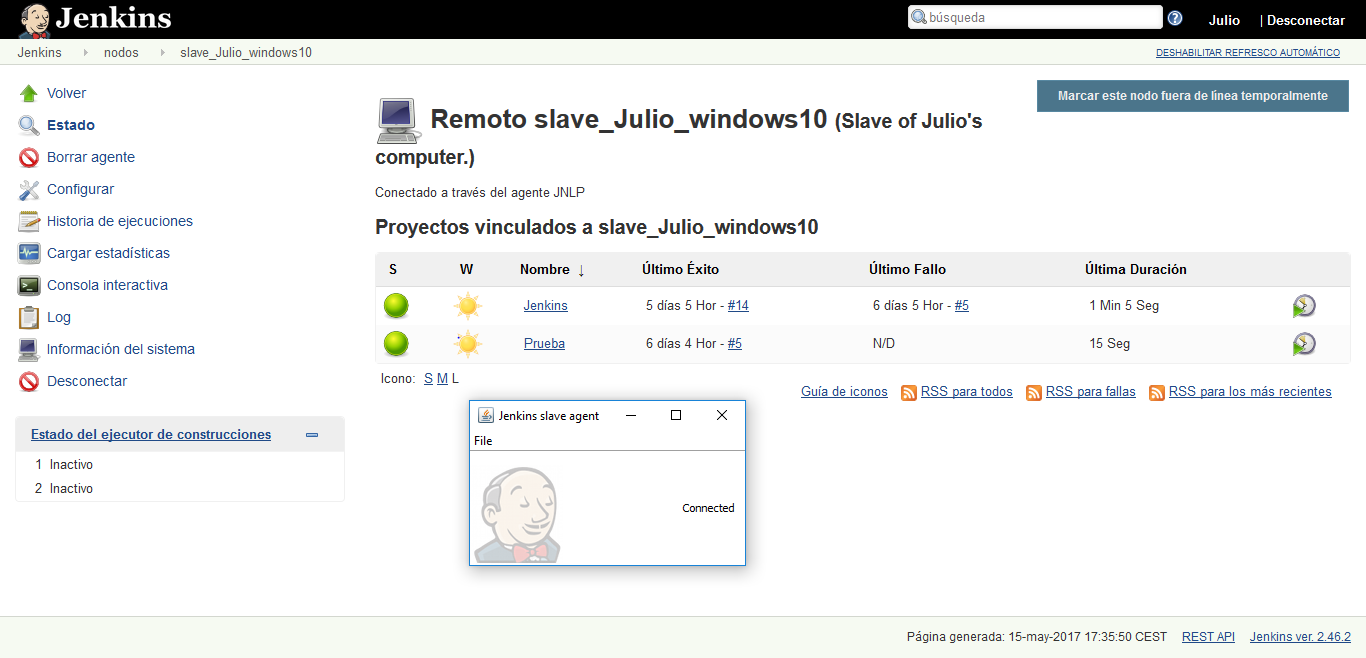
\includegraphics[width=15cm]{JavaWebStart-Jenkins-MasterSlave.PNG}
%\caption{Conexión maestro-esclavo mediante Java Web Start}
%\end{figure}

%Para esta solución el repositorio es GitLab, el servidor de integración continua es Jenkins, instalado en un computador con un sistema operativo Ubuntu Server con una arquitectura x64, el computador donde se realizan los tests sin interfaz de usuario en un computador con un sistema operativo Ubuntu Server con una arquitectura x64 y el computador donde se realizan los tests que requieren una interfaz de usuario es Windows 10 con arquitectura x64.

\begin{figure}[!h]
\centering
   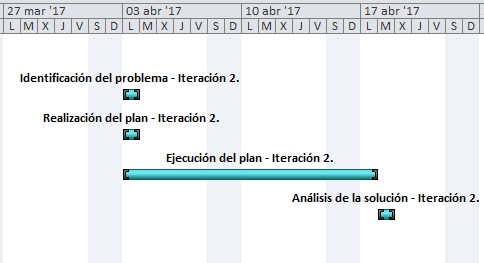
\includegraphics[width=9cm]{Diag-Gantt_It2.PNG}
\caption{Diagrama de Gantt de la iteración 2}
\end{figure}

\begin{figure}[!h]
\centering
   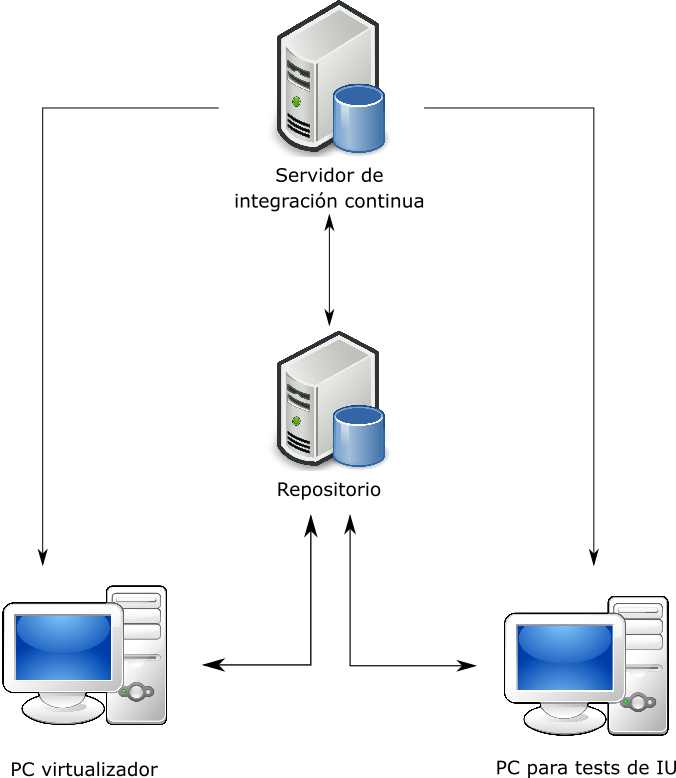
\includegraphics[width=11cm]{Arquitectura_Infraestructura_IC.png}
\caption{Versión inicial de la arquitectura e infraestructura del sistema de integración continua}
\end{figure}

\subsection{Iteración 3}

En esta tercera iteración se pretende determinar una estrategia para definir cuando debe actuar el sistema de integración continua y activar las ejecuciones correspondientes, para resolver los problemas detectados en la reunión con miembros de \ac{Madrija}, se va a seguir una metodología heurística, en concreto, la heurística IDEAL.

\subsubsection{Identificación del problema}

Se realiza una reunión con miembros de \ac{Madrija} para realizar la captura de requisitos, se validan estos requisitos y se obtiene como objetivo principal que se debe proponer una estrategia, o patrón a seguir, mediante el cual el sistema de integración continua inicie sus \textit{builds} y ejecuciones.

\subsubsection{Realización del plan}

Como paso previo a la realización del plan mediante el cual abordaremos los problemas detectados en la reunión con Madrija, se debe realizar un análisis sobre la metodología de trabajo que sigue la empresa, en especial, a su estrategia de ramificación dado que utilizan \textit{git flow}.

Una vez realizado ese estudio, se procede al análisis, diseño y desarrollo de un plan que permita abordar y solucionar los problemas identificados.

\subsubsection{Pasos a seguir en el plan}

En primer lugar se procede a analizar e investigar sobre las alternativas que ofrece la herramienta utilizada en el sistema de integración continua, con ello y teniendo en cuenta que \ac{Madrija} utiliza \textit{git flow}, encontrar así la mejor alternativa.

\clearpage

Una vez realizado el estudio y la investigación sobre las alternativas ofrecidas por la herramienta se procede a la elección de la mejor alternativa, tras realizar el estudio se detallaron dos alternativas, por una parte, mediante la detección de \textit{commits} y cambios en repositorio, es decir, se eligiría una rama, y cualquier cambio que se realizase en esa rama activaría el circuito de integración continua, por otro lado, surgió la alternativa de activar de manera nocturna todos los días el sistema de integración continua, esta segunda opción era menos convincente dado que recordaba a un ``\textit{cron}'' de Linux por lo que se ha optado por la primera opción.

\begin{figure}[!h]
\centering
   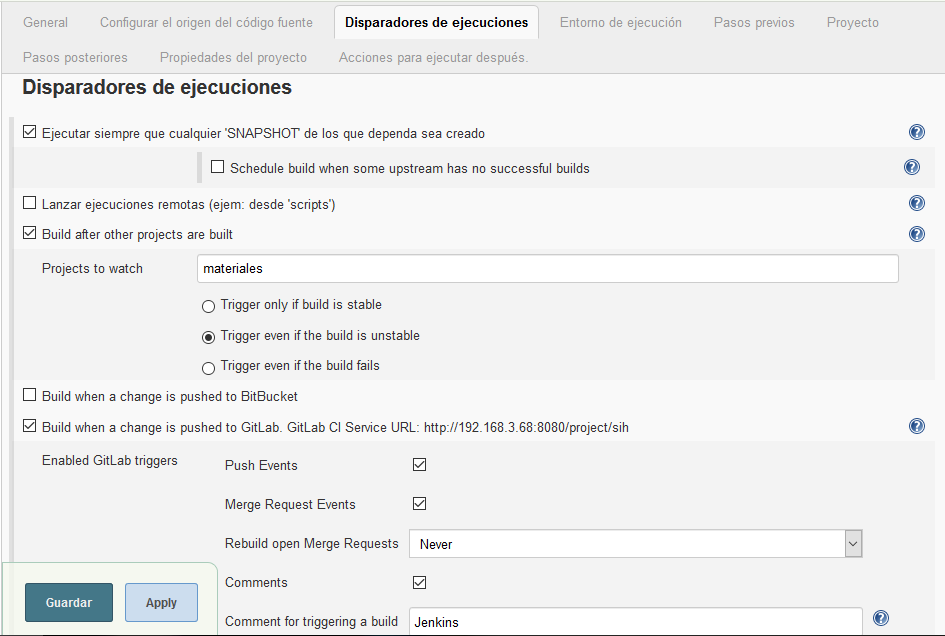
\includegraphics[width=13cm]{JenkinsSIH_Disparadores.PNG}
\caption{Detección de \textit{commit} en un proyecto Jenkins}
\end{figure}

\subsubsection{Análisis de la solución obtenida}

Se había decidido implantar una estrategia mediante la detección de \textit{commits}, es decir, si un desarrollador realizaba un \textit{commit}, de manera automática, el sistema de integración continua realizaba todas las ejecuciones involucradas, pero el plugin que realiza dicha acción tiene \textit{issues} por lo que no ha sido posible realizar esa estrategia dado que no se han solucionado los problemas.

\begin{figure}[!h]
\centering
   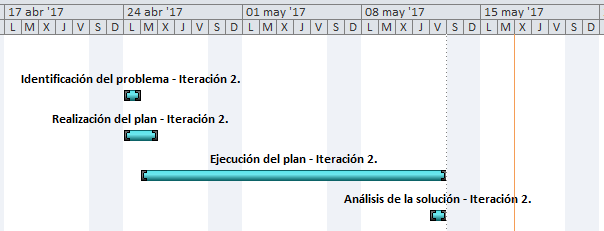
\includegraphics[width=8cm]{Diag-Gantt_It3.PNG}
\caption{Diagrama de Gantt de la iteración 3}
\end{figure}

Por lo tanto, mientras se mantenga el problema, se ha optado por otra estrategia, que consiste en realizar de manera nocturna y a diario ejecuciones automáticas de todos los proyectos y enviando así correos a los desarrolladores para que a la mañana siguiente tengan un \textit{feedback} de los cambios que realizaron el día anterior en el código fuente.

\subsection{Iteración 4}

Se pretende incorporar al sistema de integración continua la ejecución del software ``Renombrator'' el cual permite identificar y corregir palabras reservadas en el desarrollo de \ac{BBDD}.

Para realizar esta cuarta iteración, se va a seguir una metodología heurística, en concreto, la heurística IDEAL.

\subsubsection{Identificación del problema}
Se realiza una reunión con miembros de \ac{Madrija} para proceder a la captura y validación de requisitos.

Se obtiene como objetivo de esta cuarta iteración que \ac{Madrija} desarrolla software en los que trabaja con \ac{BBDD}, pero dichas \ac{BBDD} no son siempre las mismas, dado que un desarrollo puede estar destinado a trabajar con \ac{BBDD} de Oracle, otro desarrollo con \ac{BBDD} PostgresSQL, etcétera. Por lo que \ac{Madrija} ha desarrollado ``Renombrator'', un software encargado de revisar el software desarrollado referente a \ac{BBDD} y evitar el uso de palabras reservadas o carácteres incompatibles, entre otros usos.

Pero si por cada cambio que se realiza en el código, el desarrollador debe lanzar ``Renombrator'', es un trabajo repetitivo y que no produce beneficios para \ac{Madrija}, únicamente produce pérdidas en el tiempo de desarrollo.

Por lo tanto, tras una reunión con miembros de \ac{Madrija} se desea implantar ``Renombrator'' en el sistema de integración continua para que cuando algún desarrollador realice algún cambio en el código y haga \textit{commit}, el sistema de integración continua lance la ejecución de ``Renombrator'' e indique si dicha ejecución ha sido realizada de manera correcta, o si, en caso contrario, se han detectado errores que deben ser solucionados por el desarrollador.

\subsubsection{Realización del plan}
Una vez obtenidos los requisitos necesarios para esta cuarta iteración, se procede a estudiar la posibilidad y compatibilidad de implantar ``Renombrator'' en el sistema de integración continua.

\clearpage

\subsubsection{Pasos a seguir en el plan}
Dado que ``Renombrator'' es un software que no se ejecuta como test para detectar fallos, se ha decidido utilizar diferentes tecnologías para desarrollar tests mediante los cuales cuando se realice una ejecución del sistema de integración continua se verifique si el código desarrollado es correcto o si, por el contrario, necesita ser revisado dado que se haya encontrado algún error.

\subsubsection{Análisis de la solución obtenida}
Una vez finalizada la ejecución del plan de esta cuarta iteración, se realiza otra reunión con miembros de \ac{Madrija} para verificar el correcto funcionamiento de ``Renombrator'', se valida y, por lo tanto, se concluye esta cuarta iteración.

\begin{figure}[!h]
\centering
   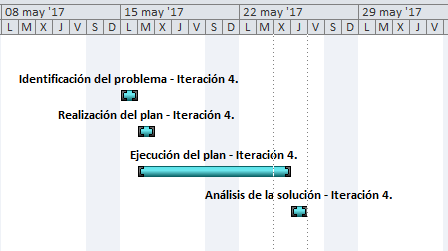
\includegraphics[width=9cm]{Diag-Gantt_It4.PNG}
\caption{Diagrama de Gantt de la iteración 4}
\end{figure}
